\documentclass{article}
\usepackage[utf8]{inputenc}
\usepackage[T2A]{fontenc}
\usepackage[english,russian]{babel}
\usepackage[left=1.5cm,right=1.5cm,top=2cm,bottom=2cm]{geometry}
\usepackage{hyperref}
\usepackage{enumitem}
\usepackage{graphicx} %библиотека для графики и картинок
\DeclareGraphicsExtensions{.pdf,.png,.jpg}


\begin{document}
% НАЧАЛО ТИТУЛЬНОГО ЛИСТА
\begin{center}
    \Large
    Федеральное государственное автономное \\
    образовательное учреждение высшего образования \\ 
    «Национальный исследовательский университет ИТМО»\\
    \vspace{0.5cm}
    \large
    
    \vspace{1cm}
    \Large
    \textbf{По дисциплине «Информационная безопасность»} \\
        Лабораторная работа №1\\
        Разработка защищенного REST API с
интеграцией в CI/CD
    \large
    \vspace{8cm}

    \begin{minipage}{.33\textwidth}
    \end{minipage}
    \hfill
    \begin{minipage}{.4\textwidth}
    
        \textbf{Студент}: \vspace{.1cm} \\
        \ Дениченко Александр Олегович P3412\\
        \textbf{Практик}:  \\
        \ Маркина Татьяна Анатольевна
    \end{minipage}
    \vfill
Санкт-Петербург\\ 2025 г.
\end{center}
\pagestyle{empty}
% КОНЕЦ ТИТУЛЬНОГО ЛИСТА 
\newpage
\pagestyle{plain}

\section*{Цель}

Получить практический опыт разработки безопасного backend-приложения с
автоматизированной проверкой кода на уязвимости. Освоить принципы защиты от OWASP Top 10 и
интеграцию инструментов безопасности в процесс разработки.
\section*{Выбранные технологии}
Java/Spring Boot, Spring Data JPA (Hibernate), H2 (in-memory), JWT (HS256), BCrypt, SAST SpotBugs, SCA Snyk, maven.

\section*{Выполение}

Проект был создан в \href{https://github.com/Alex-de-bug/security-lab-1}{GitHub} (https://github.com/Alex-de-bug/security-lab-1).
Реализовано 3 метода, где есть следующие ендпоинты:

\begin{itemize}
  \item POST /auth/login — метод для аутентификации пользователя.
  \item POST /auth/register — метод для регистрации пользователя.
  \item GET /api/data — возвращает список всех постов. Доступ только у аутентифицированных пользователей.
  \item POST /api/posts - создает новый пост от имени текущего пользователя. Доступ только у аутентифицированных пользователей.
  \item GET /api/posts/my - возвращает все посты текущего пользователя. Доступ только у аутентифицированных пользователей.
  \item Swagger UI: /swagger-ui.html
  \item H2 Console: /h2-console
\end{itemize}

\section*{Меры защиты}
\textbf{Аутентификация и сессии.} Stateless JWT Bearer (HS256), срок жизни из \texttt{86400000}, секрет был сгенерирован на сайте для генерации JWT. Пароли --- только в виде хеша BCrypt. Все запросы, кроме \texttt{/auth/**}, \texttt{/swagger-ui/**}, \texttt{/v3/api-docs/**} и \texttt{/h2-console/**}, требуют аутентификации.\\

\begin{center}
  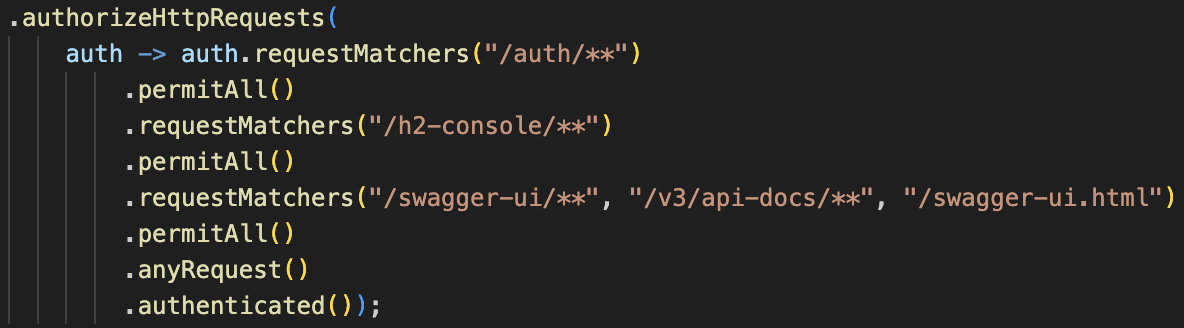
\includegraphics[width=.9\textwidth]{secur.png}
\end{center}

\textbf{SQLi.} Доступ к данным через Spring Data JPA и параметризованные запросы; отсутствует ручная конкатенация SQL.\\

\textbf{XSS.} Текстовые поля экранируются OWASP Java Encoder (утилита \texttt{Sanitizer}).\\

\section*{SAST}

Первый запуск в файле ../target/spotbugsXml(0).xml. Обнаруженные проблемы:
\\ \\
В классе ApiController (ApiController.java, строки 39–180):
\begin{itemize}
  \item Конструктор ApiController(PostService, UserRepository) сохраняет ссылку на изменяемый объект PostService в поле postService.
  \item Это может привести к тому, что внешний код, владеющий этим объектом, сможет непреднамеренно изменить внутреннее состояние контроллера.
\end{itemize}
В классе Post (Post.java, строки 14–47):
\begin{itemize}
  \item Метод getAuthor() возвращает внутренний объект author напрямую, позволяя внешнему коду изменить его.
  \item Конструктор Post(String, String, User) сохраняет ссылку на внешний объект User в поле author.
  \item Метод setAuthor(User) устанавливает напрямую ссылку на изменяемый объект User.
\end{itemize}
\textbf{Исправления, которые нужно было сделать}
\\ \\ 
Класс Post:
\begin{itemize}
    \item Добавлен безопасный метод \texttt{getAuthorInfo()}, возвращающий неизменяемый объект \texttt{UserInfo} с копией данных автора
    \item Добавлена валидация параметров с \texttt{@NotNull} и \texttt{Objects.requireNonNull()}
\end{itemize}
Класс ApiController:
\begin{itemize}
    \item Добавлена валидация входных параметров в конструкторе
    \item Заменены все вызовы \texttt{post.getAuthor().getUsername()} на безопасный \texttt{post.getAuthorInfo().getUsername()}
\end{itemize}

Итог содержится в файле  ../target/spotbugsXml(1).xml.

\section*{SCA}
Для dependecy check был выбран snyk. Была сразу поправлены все версии билиотек на новые и вот итог:
\begin{center}
  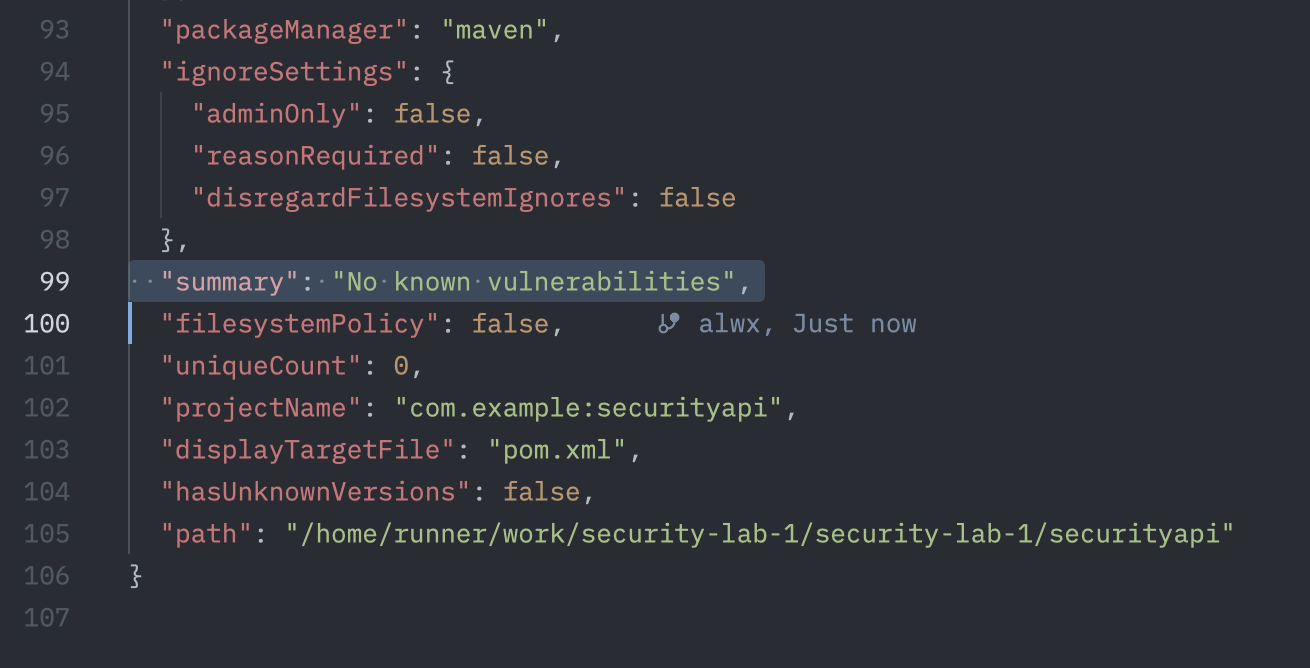
\includegraphics[width=.9\textwidth]{snyk.png}
\end{center}

Файл есть в ../target/ под названием snyk-report.json


\section*{Результаты}
Реализован защищённый REST API: аутентификация/регистрация, операции с постами, защита от XSS/SQLi, stateless JWT. Подготовлены и приложены отчёты SCA; настроена Swagger-документация.
\href{https://github.com/Alex-de-bug/security-lab-1/actions/runs/17864752066}{Последний верный CI} (https://github.com/Alex-de-bug/security-lab-1/actions/runs/17864752066)
\end{document}